
\chapter{The 3D wing}
	Before the main subject, here is some precision about the terminology:
	
	\begin{itemize}
	\item[•] $b$ is the \textbf{span}
	\item[•] $c = \frac{S}{b}$ is the \textbf{mean chord}
	\item[•] $s= \frac{b}{2}$ is the \textbf{semi span}
	\item[•] $AR = \frac{b}{c} = \frac{b^2}{S}$ is the \textbf{aspect ratio}
	\item[•] we speak about about \textbf{tapered wing} if $c_{tip} < c_{root}$ and the taper ratio is $\frac{c_{tip}}{c_{root}}$
	\item[•] we speak about \textbf{swept wing} when the leading edge and/or the trailing edge line is not $\perp$ to the flow. 
	\end{itemize}
	
	\begin{center}
	\begin{minipage}{0.4\textwidth}
	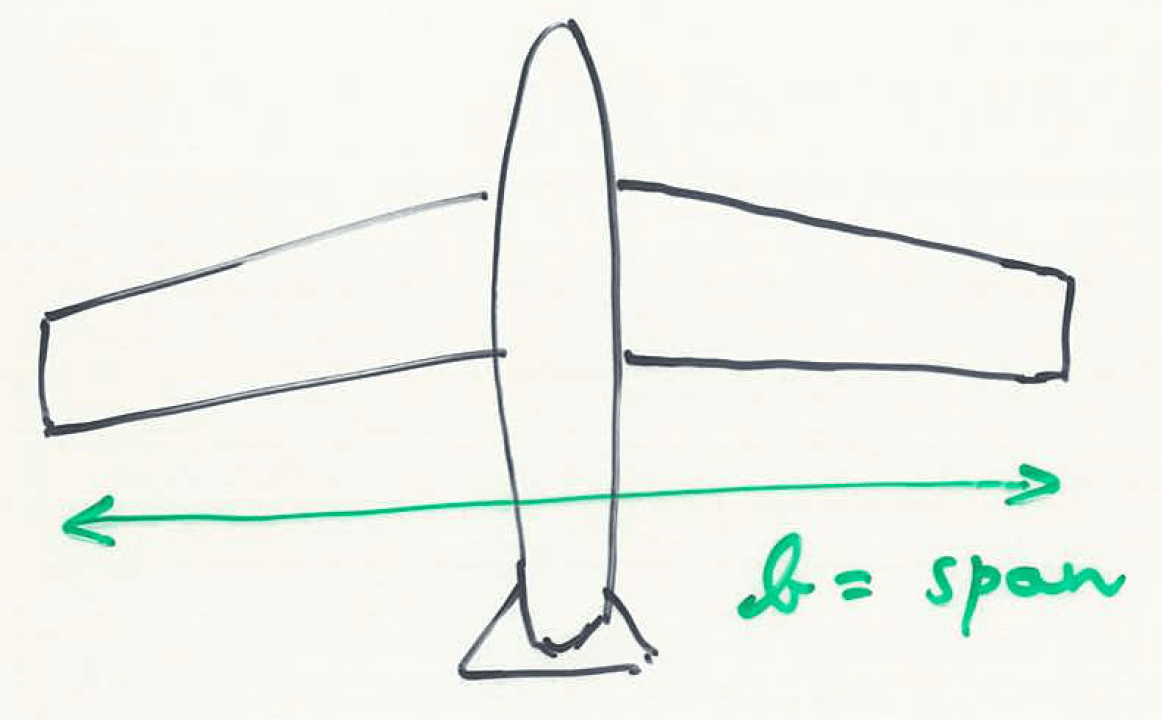
\includegraphics[scale=0.1]{ch3/1}
	\captionof{figure}{}	
	\end{minipage}
	\begin{minipage}{0.3\textwidth}
	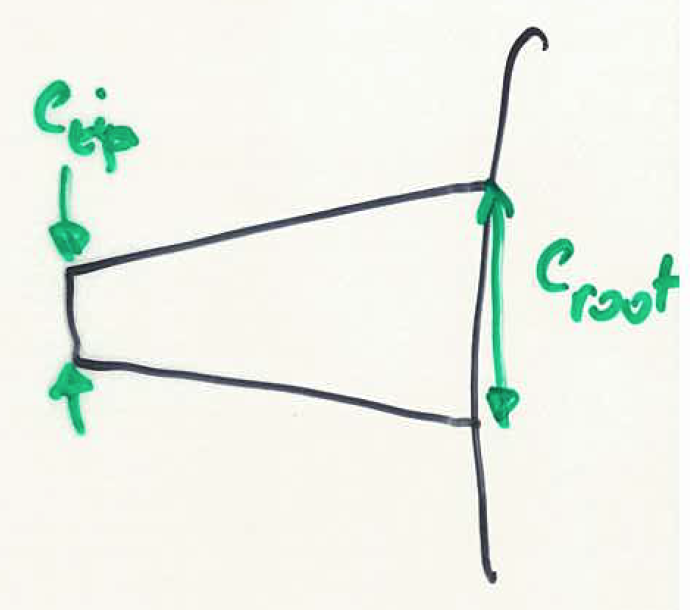
\includegraphics[scale=0.15]{ch3/2}
	\captionof{figure}{}	
	\end{minipage}
	\end{center}
	
\section{The downwash effect and the induced drag}
	\wrapfig{7}{l}{6.5}{0.1}{ch3/3}{fig:3.3}
	The 3D wing changes from the 2D case, because we have a finite span. As we know, we have a suction side and an pressure side. The thing is that because of the tip, the pressure on both side must be equal at the end of the span. This means that the pressure on the upper side must increase when going to the tip, and decrease on the lower side. This creates a pressure gradient between the root and the tip. This gradient will push the streamlines on the upper side towards the fuselage and towards the tip on the lower side. 
	
	\begin{center}
	\begin{minipage}{0.4\textwidth}
	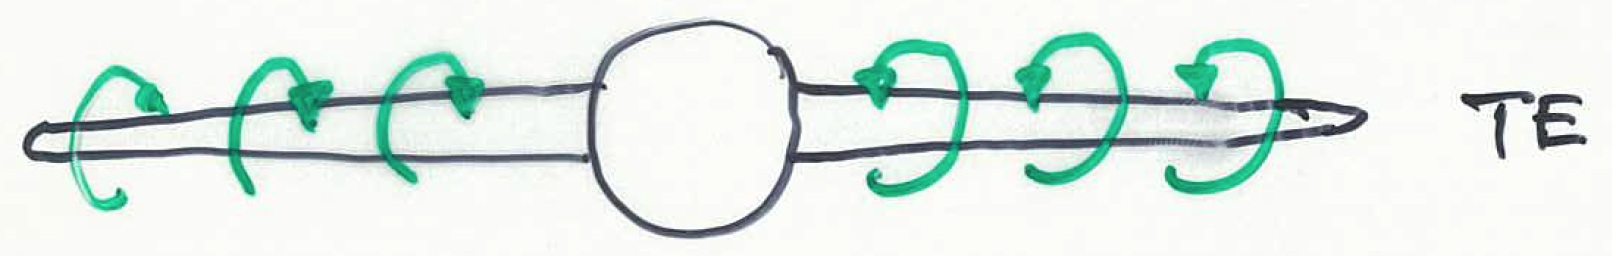
\includegraphics[scale=0.1]{ch3/4}
	\captionof{figure}{}	
	\label{fig:3.4}
	\end{minipage}
	\begin{minipage}{0.4\textwidth}
	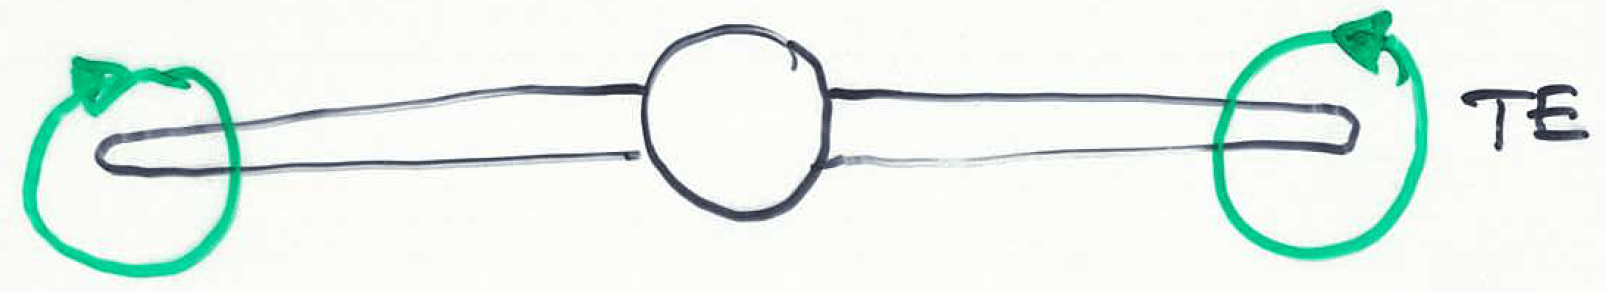
\includegraphics[scale=0.1]{ch3/5}
	\captionof{figure}{}	
	\label{fig:3.5}
	\end{minipage}
	\end{center}
	
	If we look to the trailing edge from a position downstream to the wing, this discontinuity in velocity induces an infinite series of infinitely small vortices, clockwise on the left and anti clockwise on the right wing (\autoref{fig:3.4}). In practice these vortices are unstable and result into 2 discrete vortices at the tip, the so called \textbf{wong-tip vortices or trailing vortices} (\autoref{fig:3.5}). 
	
	\wrapfig{7}{l}{6.5}{0.08}{ch3/6}{fig:3.6}
	These vortices have an effect on the neighboring flow, they induce a \textbf{downward velocity component, the downwash} $\vec{w}$. This component superposes on the incoming flow and changes the angle of attack. \autoref{fig:3.6} shows that the resulting angle is: 
	
	\begin{equation}
	\alpha _{eff} = \alpha - \epsilon
	\end{equation}
	
	where $\epsilon$ is the induced angle of attack. The decrease of $\alpha$ means a decrease in lift. Indeed, initially the flow being horizontal, the perpendicular lift was vertical. The new lift is perpendicular to the resulting flow direction, describing now an \textbf{induced drag}: 
	
	\begin{equation}
	D_i = L \sin \alpha _i \approx L\alpha _i \qquad with \qquad \alpha _i = \frac{C_L}{\pi e AR} 
	\label{eq:3.2}
	\end{equation}
	
	\wrapfig{10}{r}{5.5}{0.1}{ch3/7}{fig:3.7}
	where $e$ is the \textbf{span efficiency factor or Oswald's efficiency factor} $0.85<e<1$. If we introduce this in the definition of the induced drag, we get the Drag coefficient:
	
	\begin{equation}
	C_{D_i} =  \frac{C_L^2}{\pi e AR} .
	\end{equation}
	
	The theoretical lift curve can be obtained based on the 2D wing as \autoref{fig:3.7}. We can see that the 3D wing lift for a certain $\alpha$ corresponds to the 2D lift for the effective angle of attack $\alpha - \epsilon$. The induced angle of attack decreases with lift, at $\alpha _0$ the two curve are on the same point. Algebraically the 2D and 3D curves can be noted:
	
	\begin{equation}
	c_l = m(\alpha - \alpha _0), \qquad C_L = m(\alpha - \epsilon - \alpha _0) = m^* (\alpha - \alpha _0)
	\label{eq:3.4}
	\end{equation}
	
	where $m^*$ is the slope of the 3D lift. We can isolate this and find that:
	
	\begin{equation}
	m^* = m\left( 1 - \frac{\epsilon}{\alpha - \alpha _0} \right) = \frac{m}{1+\frac{m}{\pi e AR}} 
	\end{equation}
	
	where we used the definition \eqref{eq:3.2} and \eqref{eq:3.4} for the last result. We see that the slope is independent from $\alpha$. The total drag is the sum of the profile drag and the induced one:
	
	\begin{equation}
	C_D = C_{D_0} + kC_L^2 + C_{D_i} = C_{D_0} + C_L^2 \left( k + \frac{1}{\pi e AR}\right)
\end{equation}	 

	where $k$ is generally small compared to the other. 

	\wrapfig{8}{l}{5.5}{0.08}{ch3/8}{fig:3.8}
	With these formulas we can plot the characteristics in 3D. We can note that the maximum lift does not change so more, but there is a strong decrease in the maximum glide ratio, $C_D$ increases with $C_L$ so $\alpha$. Finally we note an increase of the stall angle but in practice this is not as large as predicted. This means also that the maximum lift decreases slightly with decreasing AR. No significant difference for the moment. 
	
	\wrapfig{5}{l}{5}{0.1}{ch3/9}{fig:3.9}
	To avoid the adverse effect which is increasing induced drag. We can use high AR or add winglet on the tip, a kind of end plate that forces a vertical diffusion of the tip vortex, reducing drag. They have to be carefully designed to not increase the viscous drag. 
	
\subsection{Variation of the drag during the flight}
	We found the drag coefficient on the wing but we have also the drag coming from the fuselage, etc. These part does not contribute in lift so they  are called \textbf{parasite drag}. Let's compute the total drag using the coefficient definition:
	
	\begin{equation}
	\begin{aligned}
	D &= C_D \frac{1}{2} \rho _\infty v_\infty ^2 S = C_{D_0} \frac{1}{2} \rho _\infty v_\infty ^2 S + \left(k +\frac{1}{\pi e AR} \right)\frac{L^2}{( \frac{1}{2} \rho _\infty v_\infty ^2 S)^2} \frac{1}{2} \rho _\infty v_\infty ^2 S \\
	&= k_1 v_\infty ^2 + k_2 v_\infty^2.
	\end{aligned}
	\label{eq:3.7}
	\end{equation}
	
	If the plane is in stationary flight, the lift is equal to the weight W of the plane. One can write, introducing a and b bigger than the previous coefficients in order to take into account the drag furnished  by the whole plane:
	
	\begin{equation}
	\begin{aligned}
	k_1 &= C_{D_0} \frac{1}{2} \rho _\infty S = a \frac{1}{2} \rho _\infty S\\
	k_2 &= \left(k +\frac{1}{\pi e AR} \right)\frac{W^2}{\frac{1}{2} \rho _\infty  S}  = b \frac{W^2}{\frac{1}{2} \rho _\infty  S}
	\end{aligned}
	\end{equation}
	
	where the terms $k_1$ and $k_2$ represent the profile drag and the induced drag. An important conclusion is that the profile drag increases with the square of velocity while the induced drag does the contrary. We can find a point of minimum drag by canceling D in \eqref{eq:3.7}:
	
	\begin{equation}
	v_{min}^4 = \frac{k_2}{k_1} \qquad \Rightarrow D_{min} = 2\sqrt{k_1k_2} = 2W\sqrt{ab}.
	\end{equation}
	
	\wrapfig{8}{r}{4}{0.12}{ch3/10}{fig:3.10}
	This is only dependent of the weight. This minimum velocity gives the lower limit of the region where the plane is well controllable. Indeed, for a small decrease, we increase the drag that will decrease the velocity and so on. This is an unstable situation. Note that the minimal velocity is higher than the stall velocity. Remark that the dashed curves on the graph take into account the separation occuring due to the drag. We find two solution, this is logical as in $c_l$ we can have the same lift with two $\alpha$. 
	
	
\section{Prandtl lifting line theory}
\subsection{Introduction : vortex lines and law of Biot-Savart}
\subsubsection{Vortex lines and the Helmholtz theorems}
	\wrapfig{6}{l}{7}{0.12}{ch3/11}{fig:3.11}
	The seen free vortex is characterized by circular streamlines around a certain point P. In this point the vorticity is concentrated such that the circulation around the contours that don't contain the point are null. If we consider several planes above each other containing a 2D free vortex, the point P form a line called \textbf{vortex line or vortex filament}. The circulation on each point of that line have the same circulation. 
	
	\begin{center}
	\theor{\textbf{Helmholtz theorems}\\
	\begin{itemize}
	\item[•] Along a vortex line, the circulation must be constant.
	\item[•] A vortex line cannot finish in the flow but must continue to the edges of the flow or form a closed contour. 
	\end{itemize}
	 }
	\end{center}
	
	\wrapfig{6}{l}{6.5}{0.06}{ch3/13}{fig:3.13}
	This line can be a random line with bending. Now if one places an infinite number of vortex lines besides each other, we get a \textbf{vortex sheet}. For the total circulation to be finite, the circulations must be infinitely small, but can vary from one line to the other. The circulation of the vortex sheet is calculated as:
	
	\begin{equation}
	\Gamma = \int _a ^b d\Gamma = \gamma \, ds \qquad and \qquad \Delta v_t = \gamma 
	\end{equation}
	
	the normal component of the velocity is continuous while the tangential one varies as in the last equation. 
	
\subsubsection{Law of Biot-Savart}
	\wrapfig{6}{r}{4}{0.1}{ch3/12}{fig:3.12}
	This law gives the induced velocity in a certain point P cause by an elementary piece $d\vec{l}$ of the filament: 
	
	\theor{
	\textbf{Law of Biot-Savart}
	\begin{equation}
	d\vec{v} = \frac{\Gamma }{4\pi} \frac{d\vec{l}\times r}{|r|^3}
	\end{equation}
	}
	
	\ \\ With analogy to electrical wire where we have a current intensity that induces a magnetic field on point P: $d\vec{B} = \frac{\mu I }{4\pi} \frac{d\vec{l}\times r}{|r|^3}$. 
	
\subsubsection{Application of Biot-Savart to a vortex filament}
	\wrapfig{10}{l}{5}{0.1}{ch3/14}{fig:3.14}
	The law tells us that at point P:
	
	\begin{equation}
	\vec{v} = \frac{\Gamma }{4\pi}\int _{-\infty}^{+\infty} \frac{d\vec{l}\times r}{|r|^3}.
	\end{equation}
	
	Looking to the figure, we see that $d\vec{l} \times \vec{r} = Rdl \vec{1}_n$ defined on the figure. So $\vec{v} = v \vec{1}_n$. Let's define the length $l$ beginning from the piercing point on the surface until the $d\vec{l}$. We can graphically see that: 
	
	\begin{equation}
	l  = -R \coth \theta \Rightarrow dl = \frac{R}{\sin ^2\theta} d\theta, \qquad r = \frac{R}{\sin \theta} 
	\end{equation}
	
	Replacing all this we get:
	
	\begin{equation}
	v = \frac{\Gamma}{4\pi} \int _{0}^{\pi} \frac{R^2}{\sin^2 \theta } \frac{\sin ^3 \theta}{R^3} d\theta \qquad \Rightarrow v = \frac{\Gamma}{2\pi R}.
	\end{equation}
	
	This is the velocity distribution of the 2D free vortex. 
	
\subsection{Prandtl lifting line formula}
	\wrapfig{10}{l}{7}{0.08}{ch3/15}{fig:3.15}
	The idea is to represent the 3D wing by means of vortex filaments. On the figure we have the \textbf{horseshoe vortex} where the x direction continues to infinity to satisfy the Helmholtz condition and the y direction extends from $-b/2$ to $b/2$ and represents the two wings. This last is the bound vortex and the one in x direction represents the tip vortices. The problem with the representation is that we have a constant circulation while we have seen that the lift decreases when going to the tips. 
	
	\wrapfig{10}{r}{5}{0.1}{ch3/16}{fig:3.16}
	Let's try to compute the downwash velocity on a point from the bound vortex. The law of Biot-Savart has 3 contributions: 
	
	\begin{equation}
	\vec{v} = \int _{-\infty} ^{-b/2} \dots + \int _{-b/2} ^{b/2} \dots + \int _{b/2}^{\infty}.
	\end{equation}
	
	The second integral vanishes as dl and r are parallel, the two others were computed at the previous section. Pay attention that we have to take half the contribution as the integral is not $-\infty,+\infty$:
	
	\begin{equation}
	\vec{v}(y) = \left(\frac{\Gamma}{4\pi R} + \frac{\Gamma}{4\pi R^*} \right) \vec{1}_n
	\end{equation}
	
	We can see that the velocity is infinity at the tips and minimum at the middel. This is clearly not the reality. 
	
	\begin{center}
	\begin{minipage}{0.4\textwidth}
	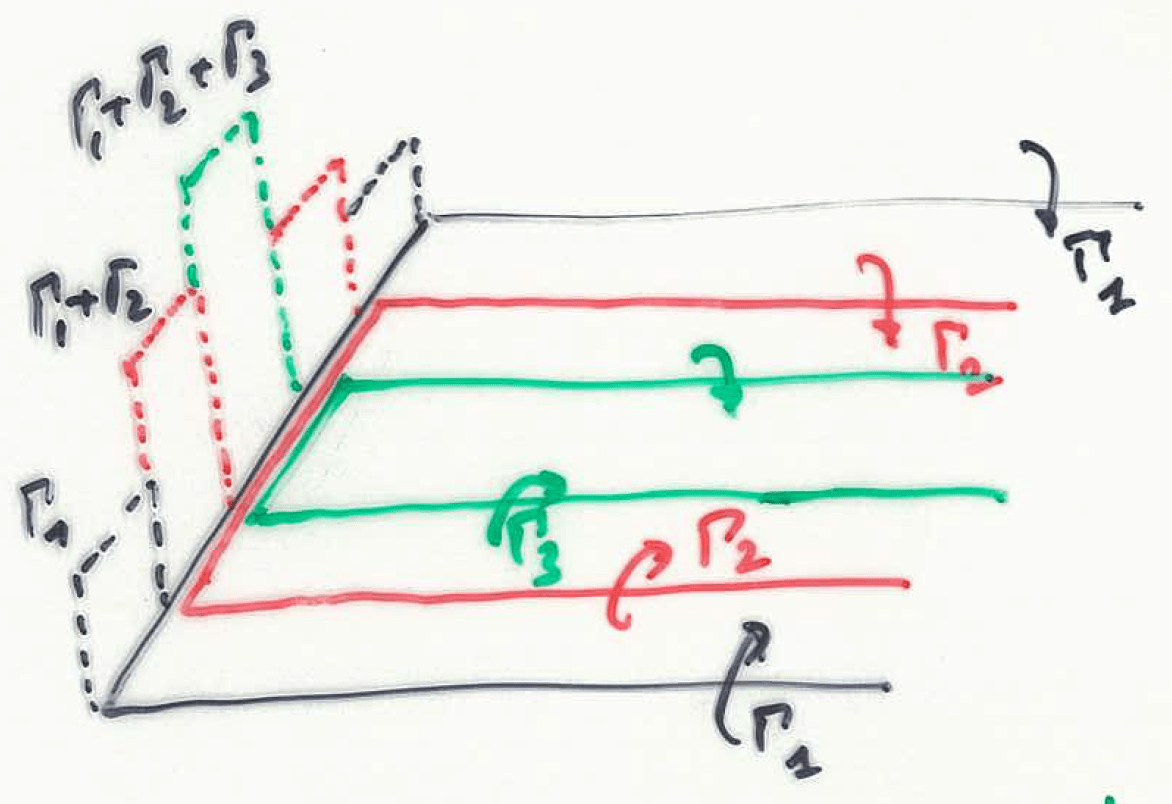
\includegraphics[scale=0.15]{ch3/17}
	\captionof{figure}{}	
	\label{fig:3.17}
	\end{minipage}
	\begin{minipage}{0.4\textwidth}
	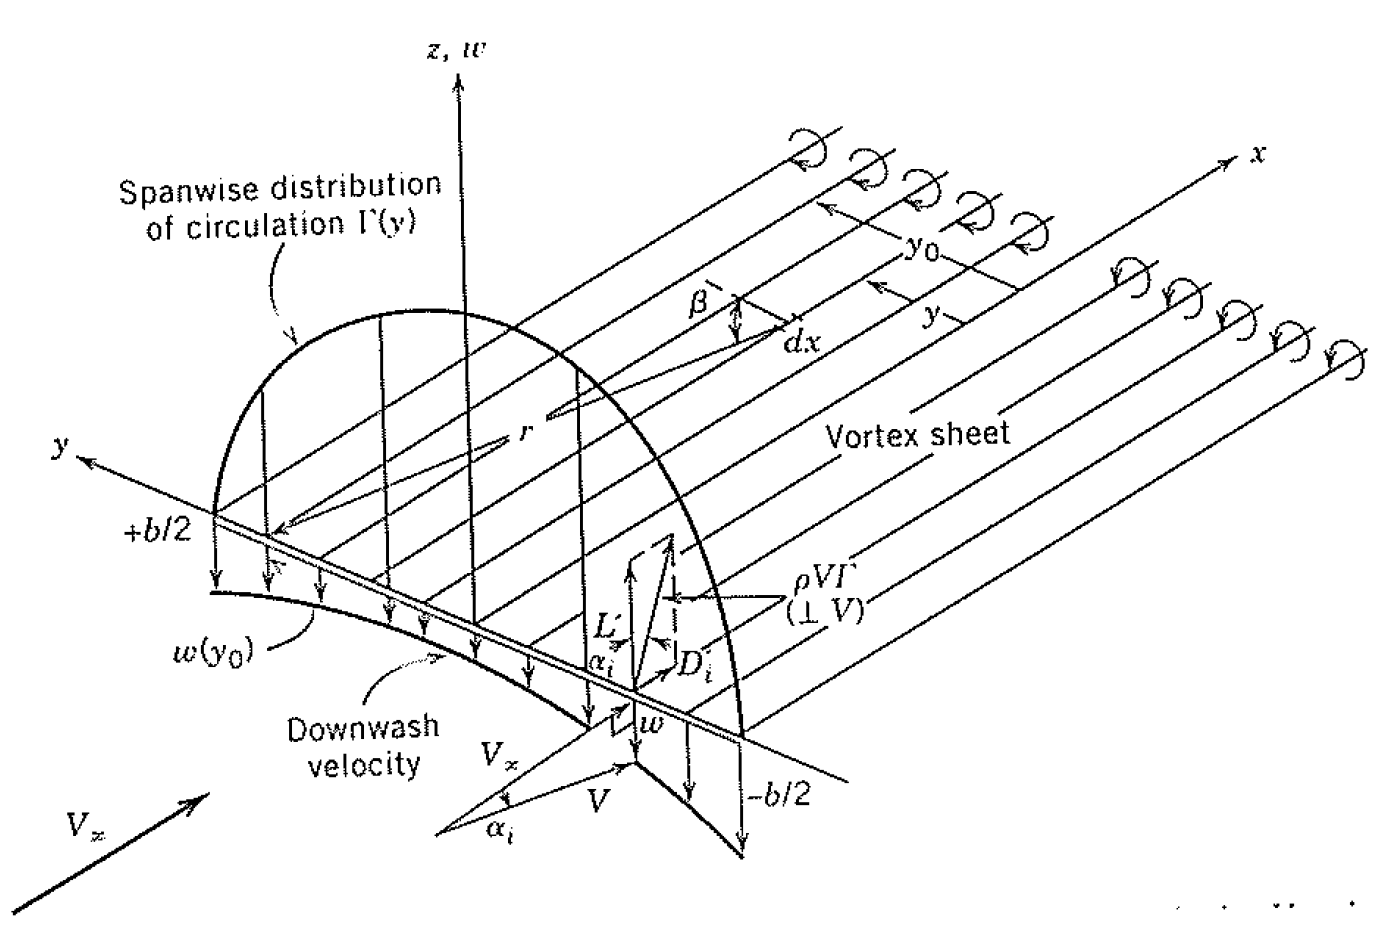
\includegraphics[scale=0.12]{ch3/18}
	\captionof{figure}{}	
	\label{fig:3.18}
	\end{minipage}
	\end{center}
	
	The solution is to superpose the horseshoes with bound vortices with different length. \autoref{fig3.17} shows how the superposition affects the circulation on the wing. If now we let tend the number of superimposed horseshoe vortices to infinity, we will get a vortex sheet as represented on \autoref{fig:3.18}. The continuously varying circulation on the wing is no longer constant and this corresponds better with the reality. 
	
	\wrapfig{10}{l}{5}{0.08}{ch3/19}{fig:3.19}
	Consider this figure, we will try to compute the downwash velocity by considering a large but finite number of vortices of circulation $d \Gamma$ for each. We have 3 regions to consider with our basic formula:
	
	\begin{itemize}
	\item[•] $y<0$: $d\vec{v}(y_0) =  \frac{d \Gamma}{4\pi (y_0-y)}\vec{1}_n$
	\item[•] $0<y<y_0$: $d\vec{v}(y_0) = \frac{d \Gamma}{4\pi (y_0-y)}\vec{1}_N = \frac{-d \Gamma}{4\pi (y_0-y)}\vec{1}_n$
	\item[•] $y_0<y$: $d\vec{v}(y_0) =  \frac{d \Gamma}{4\pi (y-y_0)}\vec{1}_n = \frac{-d \Gamma}{4\pi (y_0-y)}\vec{1}_n$  
	\end{itemize}
	
	We can see that the three formulas are the same if we take $\Gamma < 0$ for $y>0$. We can so write the total contribution and its extension to the infinite number of lines:
	
	\begin{equation}
	\vec{v} = \left[ \sum \frac{d\Gamma}{4\pi (y_0 - y)} \right] = \left[ \int _{-b/2}^{b/2} \frac{d\Gamma}{4\pi (y_0 - y)} \right]
	\end{equation}
	
	\wrapfig{10}{l}{5}{0.15}{ch3/20}{fig:3.20}
	The induced angle of attack is then given by:
	
	\begin{equation}
	\tan \alpha _i \approx \alpha _i = \frac{v(y_0)}{v_\infty} = \frac{1}{4\pi v_\infty} \int _{-b/2} ^{b/2}\frac{d\Gamma}{y_0-y}.
	\label{eq:3.18}
	\end{equation}
	
	Now let's denote $\alpha _{eff} = \alpha - \epsilon$. We know that the theory says $c_l = 2\pi (\alpha _{eff}(y_0)- \alpha _0(y_0))$, and using the definition of $c_l$ and the Kutta-Jukowski for $L(y_0)$ we get:
	
	\begin{equation}
	\begin{aligned}	
	&c_l = \frac{L(y_0)}{\frac{1}{2}\rho_\infty v_\infty ^2 c(y_0)} = \frac{\rho _\infty v_\infty \Gamma (y_0)}{\frac{1}{2}\rho_\infty v_\infty ^2 c(y_0)} = \frac{\Gamma (y_0)}{\frac{1}{2}v_\infty ^2 c(y_0)} \\
	&\Rightarrow \alpha _{eff} = \frac{\Gamma (y_0)}{\pi v_\infty c(y_0)} + \alpha _0(y_0)
	\end{aligned}
	\end{equation}
	
	Combining all the result, we can compute the $\alpha$: 
	
	\begin{center}
	\theor{
	\textbf{Fundamental equation of Prandtl's lifting line theory}
	\begin{equation}
	\alpha(y_0) = \frac{\Gamma (y_0)}{\pi v_\infty c(y_0)} + \alpha _0(y_0) + \frac{1}{4\pi v_\infty} \int _{-b/2}^{b/2} \frac{d\Gamma}{y_0 - y}. 
	\end{equation}		
	}
	\end{center}
	
	The only unknown in this equation is the circulation, the integral is not very easy to handle, we will see how to compute it in next section. 
	

\subsection{The elliptic lift distribution (application type II)}
	Before starting, let's do a summery  of what we have done. The line theory for a given wing is an integro-differential equation for $\Gamma (y_0)$, so the solution is $\Gamma (y_0)$. Then we can compute the local and total lift by:
	
	\begin{equation}
	L'(y_0) = \rho _\infty v_\infty \Gamma (y_0) \qquad L = \int _{-b/2}^{b/2} L'(y)\, dy
	\end{equation}
	
	and the local and total induced drag: 
	
	\begin{equation}
	D'_i (y_0) = \Gamma (y_0) \epsilon (y_0) \qquad D_i = \int _{-b/2}^{b/2} D_i'(y)\, dy
	\end{equation}
	
	Now if we can assume a lift distribution on the wing, we can directly go throw the last equations. The elliptic circulation distribution is written:
	
	\begin{equation}
	\Gamma (y) = \Gamma (y_0) \sqrt{1-\left( \frac{y}{b/2} \right)^2}.
	\end{equation}
	
	where $\Gamma _0$ is the circulation in the plane of symmetry. Let's compute the velocity:
	
	\begin{equation}
	v(y_0) = \frac{1}{4\pi} \int _{-b/2}^{b/2} \frac{d\Gamma }{y_0 - y} = \frac{\Gamma _0}{2b} = cst \qquad \Rightarrow \epsilon = \alpha _i = \frac{v(y_0)}{v_\infty} = \frac{\Gamma _0}{2b v_\infty} = cst.
	\end{equation}
	
	where we used the transformation $y = b/2 \cos \theta$. We see that the induced angle of attack is constant along the span. We can compute $L'(y)$: 
	
	\begin{equation}
	L'(y) = \rho v_\infty \sqrt{1-\left( \frac{y}{b/2} \right)^2}.
	\end{equation}
	
	On the other hand we can use \eqref{eq:3.4} to express the lift as: 
	
	\begin{equation}
	L'(y) = m (\alpha - \alpha _i - \alpha _0) \frac{1}{2} \rho _\infty v_\infty ^2 c
	\end{equation}
	
	Combining the equations we get: 
	
	\begin{equation}
	(\alpha - \alpha _i - \alpha _0) c = \frac{2\Gamma _0}{v_\infty} \sqrt{1-\left( \frac{y}{b/2}\right)^2}. 
	\end{equation}
	
	Note that if the left hand side is constant, the equation is satisfied for an \textbf{elliptic platform}. Since $\alpha _i$ is already constant, the whole term is constant only if the geometric angle of attack is constant and the profile does not change along the span. Since $C_{d_i} = C_L \alpha _i$, we can make the same analysis for the drag. \\
	
	On the other hand, if the platform is non elliptic, since m varies little, the different angles must vary too. This is done by introducing a \textbf{twist} in the wing so that $\alpha$ varies. The lift coefficient is obtained by integration of the local lift:
	
	\begin{equation}
	\frac{1}{\frac{1}{2}\rho v_\infty ^2 S} \int _{-b/2}^{b/2} L'(y) \, dy = \frac{\Gamma _0\pi b}{2v_\infty S} = \frac{\Gamma _0 \pi}{2bv_\infty} AR.
	\end{equation}
	 
	 Combination of this and what we found for $\alpha _i$ in this section we get:
	 
	 \begin{equation}
	 \alpha _i = \frac{C_L}{\pi AR}
	 \end{equation}
	 
	 which is what we defined at the beginning of the chapter but for $e =1$ (span efficiency factor). The induced drag is given by:
	 
	 \begin{equation}
	 D_i'(y) = L'(y) \alpha _i \qquad \Rightarrow C_{D_i} = C_L \alpha _i = \frac{C_L^2}{\pi AR}.
	 \end{equation}
	 
\subsection{Wings with arbitrary distribution of the circulation}
	in this case we don't know a priori the lift distribution, we assume a serie:
	
	\begin{equation}
	\Gamma = \sum _{n=1} ^N A_n \sin (n\theta).
	\end{equation}
	
	Substitution of this in the Prandtl's fundamental equation gives:
	
	\begin{equation}
	\alpha (\theta _0) = \frac{1}{\pi v_\infty c(\theta _0)} \sum _n A_n \sin (n\theta_0) + \alpha_0(\theta _0) + \frac{1}{2\pi v_\infty b} \sum _n A_n n \int ^0_\pi \frac{\cos (n\theta)d\theta}{\cos \theta _0 - \cos \theta}
	\label{eq:3.32}
	\end{equation}
	
	where we recognize the Glauert integral. We have here 1 equation for N unknowns $A_1, \dots, A_N$. We can find a solution by considering N equations for N points distributed along the span. Let's calculate the lift coefficient as for the previous section, by integrating:
	
	\begin{equation}
	C_L = \frac{1}{\frac{1}{2}v_\infty S} \int _{-b/2}^{b/2} \Gamma (y) \, dy = \frac{b}{u_\infty S} \sum _n \int _0 ^\pi A_n \sin (n\theta) \sin \theta \, d\theta = \frac{\pi b A_1}{2Sv_\infty}. 
	\end{equation}
	
	For the induced drag we have: 
	
	\begin{equation}
	C_{D_i} = \frac{1}{\frac{1}{2} v_\infty S} \int _{-b/2} ^{b/2} \Gamma (y)\alpha _i \, dy. 
	\end{equation}
	
	Using \eqref{eq:3.18}, we can express $\alpha _i (\theta _0)$ as:
	
	\begin{equation}
	\alpha _i (\theta _0) = \frac{1}{2\pi v_\infty b} \int ^{0}_{\pi} \frac{\frac{d\Gamma }{d\theta}}{\cos \theta _0 - \cos \theta} \, d\theta = \frac{1}{2\sin \theta _0 v_\infty b} \sum _n A_n n \sin (n \theta _0)
	\end{equation}
	
	we can say that the induced drag is:
	
	\begin{equation}
	C_{D_i} = \frac{1}{2v_\infty ^2 S} \int _0 ^\pi \sum _n \sum _k A_n A_k \sin (n\theta) \sin (k\theta) \, d\theta = \frac{\pi}{4v_\infty ^2 S} \sum _n A_n ^2 n
	\end{equation}
	
	and using the lift coefficient:
	
	\begin{equation}
	C_{D_i} = \frac{C_L^2}{\pi AR}  \left(1+\sum _{n=2} n \left(\frac{A_n}{A_1}\right)^2 \right) \qquad \Rightarrow e = \frac{1}{1+\sum _{n=2} n \left(\frac{A_n}{A_1}\right)^2} = \frac{1}{1+\delta}
	\end{equation}
	
	where $\delta $ is the \textbf{induced drag factor}, since it is always positive, $e<1$. 
	
\subsubsection{Application 1: tapered wing}
	
	\begin{center}
	\begin{minipage}{0.4\textwidth}
	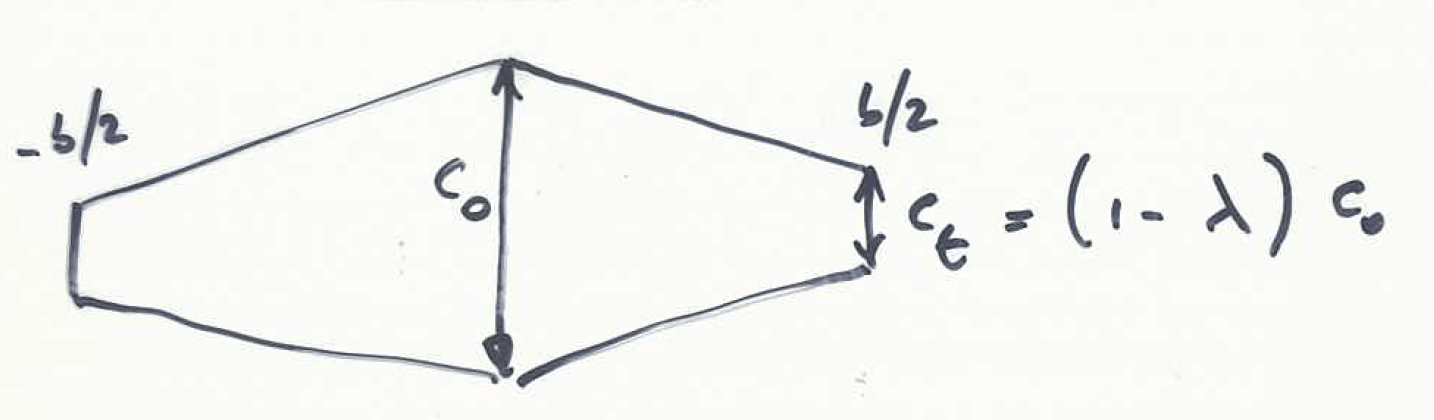
\includegraphics[scale=0.05]{ch3/21}
	\captionof{figure}{}	
	\label{fig:3.21}
	\end{minipage}
	\begin{minipage}{0.22\textwidth}
	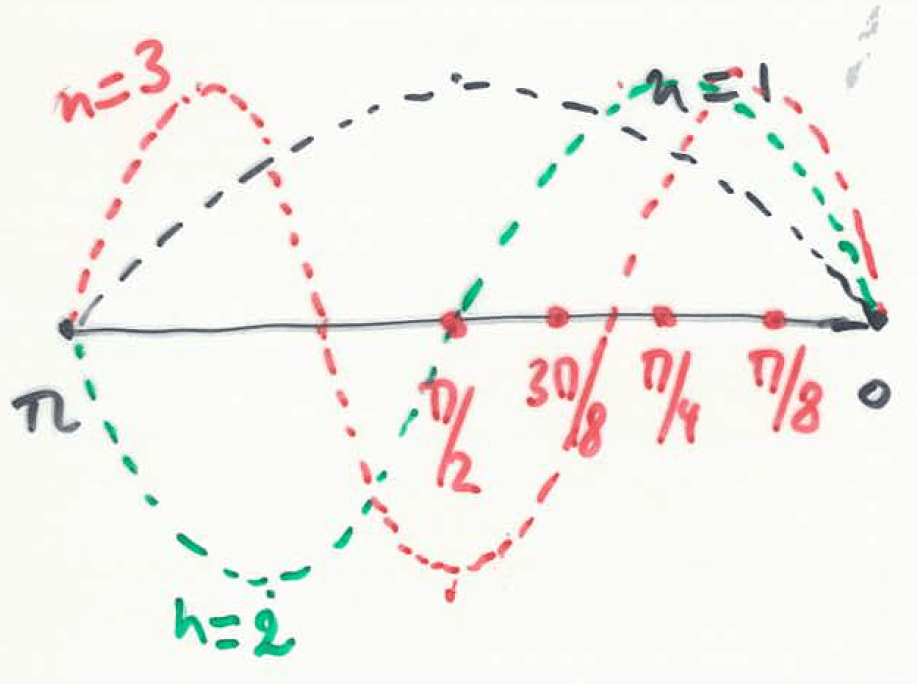
\includegraphics[scale=0.02]{ch3/22}
	\captionof{figure}{}	
	\label{fig:3.22}
	\end{minipage}
	\end{center}

	Same 2D profile along the span and no twist. Because of the symmetry, it is obvious that the pair n will have no contribution. Let's go until 7:
	
	\begin{equation}
	\Gamma = A_1\sin \theta + A_3\sin 3\theta + A_5\sin 5\theta + A_7\sin 7\theta.
	\end{equation}
	
	To determine the coefficient we have to apply \eqref{eq:3.32} to 4 points. Let's take half the span because of symmetry: $\theta = \pi /8, \pi /4, 3\pi /8, \pi /2$. Since the 2D profile is constant, $\alpha _0$ is independent of $\theta$, same for $\alpha$ since there are no twist. 
	
	\begin{center}
	\begin{minipage}{0.4\textwidth}
	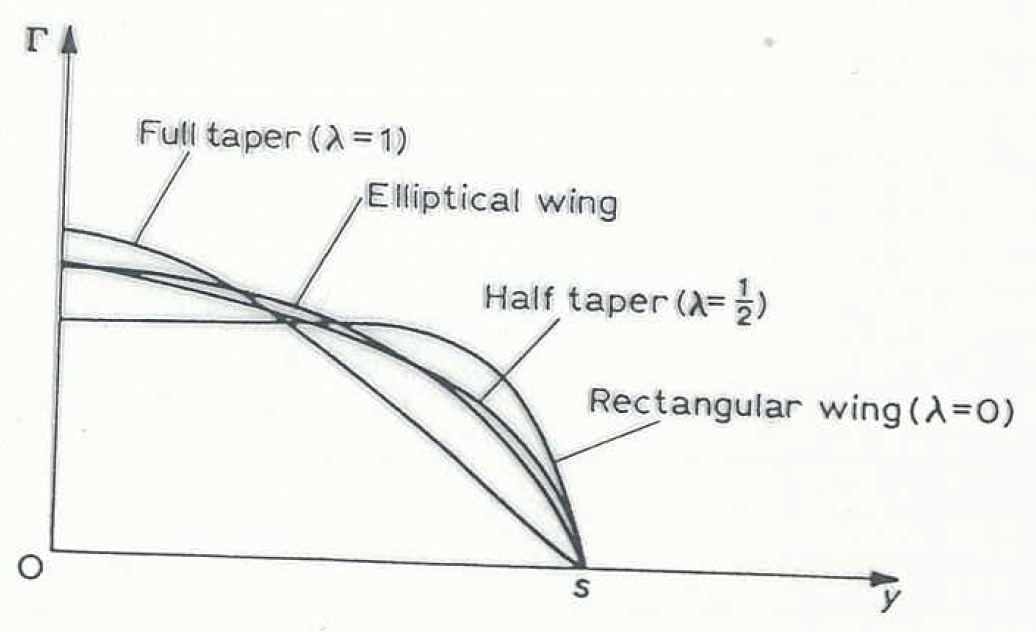
\includegraphics[scale=0.15]{ch3/23}
	\captionof{figure}{}	
	\label{fig:3.23}
	\end{minipage}
	\begin{minipage}{0.22\textwidth}
	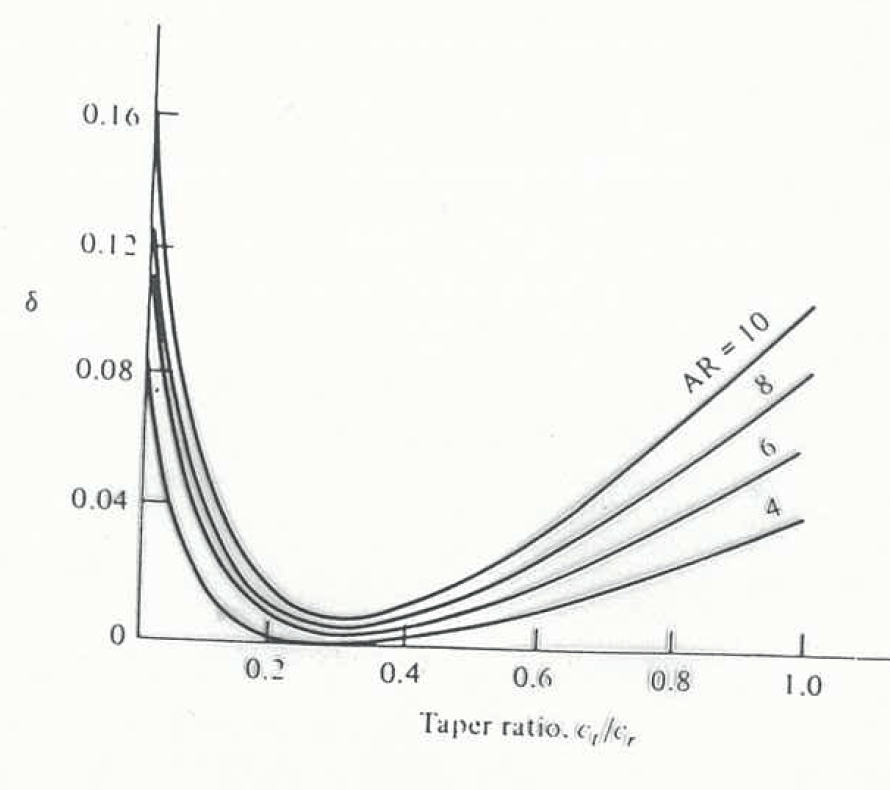
\includegraphics[scale=0.12]{ch3/24}
	\captionof{figure}{}	
	\label{fig:3.24}
	\end{minipage}
	\end{center}
	
	After some calculation one find a circulation distribution as in \autoref{fig:3.23}, where $\lambda$ is defined such that $c_t = (1- \lambda) c_r$. $\lambda = 0$ corresponds to a rectangular wing and $\lambda = 1$ is the triangular one. Note that the figure also represents the lift. The lift coefficient no, because it becomes larger at the tips due to $c\searrow$. On \autoref{fig:3.24} is represented the induced drag coefficient $\delta$. We see that it is always possible to find the taper ratio to have the minimum drag. Most of the planes use tapered wings since it is more simple to produce than elliptic wing. 
	
\subsubsection{Application 2: a wing with twist}
	We have to distinguish: 	
	\begin{itemize}
	\item[•] \textbf{Geometrical twist}: the slope of the chord varies along the span, if $\alpha$ decreases from root to top, we speak about \textbf{geometrical washout}. 
	\item[•] \textbf{Aerodynamic twist}: in this case we play with the geometry of the 2D airfoil, the camber. If the camber decreases from root to tip, we speak about \textbf{aerodynamic washout}. 
	\end{itemize}
	
	\ \\ For the calculations, it is similar to the tapered wing but this time $\alpha$ and/or $\alpha _0$ varies with the points. In general, one finds that the geometrical washout decreases $\delta$ and therefor the induced drag, except at very low lift coefficients (high velocity the drag is already not so important). 
	
\subsubsection{Numerical treatment}
	Instead of series, we can use the numerical treatment. We divide the wing in a number of stations spread along the span. For a given $\alpha$, one assumes a value for $\Gamma$ in each of the stations. This allows to calculate the induced angle of attack via: 
	
	\begin{equation}
	\alpha _i(\theta _0) = \frac{1}{4\pi v_\infty} \int _{-b/2}^{b_2} \frac{d\Gamma}{y_0- y}
	\end{equation}
	
	where the integral is now computed numerically. Knowing this angle, we can use the 2D lift curve to find the local lift coefficient. On the other hand we have from Kutta-Joukowski:
	
	\begin{equation}
	c_l (\theta _0) = \frac{\Gamma (\theta _0)}{\frac{1}{2}v_\infty c(\theta _0)}
	\end{equation}
	
	\wrapfig{9}{l}{5.5}{0.12}{ch3/25}{fig:3.25}
	where we know $c_l$, so we get a new $\Gamma (\theta _0)$ different from the postulated one. This leads to a new circulation:
	
	\begin{equation}
	\Gamma = \Gamma _{old} + \omega (\Gamma _{new} - \Gamma _{old})
	\end{equation}
	
	where $\omega$ is an underrelaxation factor to stabilize the method ($\approx 0.05$). The new $\Gamma$ gives a new distribution of the induced angle and we repeat the method until the convergence. This method can be used at stall, since we make use of the 2D curves. One has to be cautious since there is important 3D effects when separation. 
	\ \\
	
	\wrapfig{10}{l}{6}{0.12}{ch3/26}{fig:3.26}
	The lifting line theory gives good results for wings of more or less rectangular shape and average to high AR. For higher velocities however one frequently uses swept wings: the entire wing is placed at an angle with regard to the flow direction. Our theory is not as accurate as needed for the shapes shown on the figure. We have to use the \textbf{lifting surface theory}. 